
%%%%%%%%%%%%%%%%%%%%%%%%%%%%%%%%%%%%%%%%%%%%%%%%%%
\begin{frame}[fragile]{Our Starting Point}
\begin{itemize}
\item Business Software
\item Very poor code quality
\item Planned changes for a module:
\begin{itemize}
\item Bugfixing
\item new features
\item better tests
\end{itemize}
\end{itemize}

$\Rightarrow$ A restructuring was required
\end{frame}

%%%%%%%%%%%%%%%%%%%%%%%%%%%%%%%%%%%%%%%%%%%%%%%%%%
\begin{frame}[fragile]{The Domain}
\begin{itemize}
\item Financial mathematical software
\end{itemize}

\begin{itemize}
\item Calculate for a bank account for each month:
\begin{itemize}
\item Balance at the last day of the month (ultimo)
\item Average balance of the month
\end{itemize}
\end{itemize}

\end{frame}


%%%%%%%%%%%%%%%%%%%%%%%%%%%%%%%%%%%%%%%%%%%%%%%%%%
\begin{frame}[fragile]{Problems of the Existing Code Structure}
\begin{minipage}{.45\paperwidth}
\begin{itemize}
\item Code writes values into separate data objects (\glqq Push\grqq{})
\item Multiple writing operations for one value
\item Parts of  the code access previously written values
\item Code is driven by the view \textbf{from the inside}: What do I need to do in summary to be able to deliver a set of result values?
\end{itemize}
\end{minipage} \hfill
\begin{minipage}{.45\paperwidth}
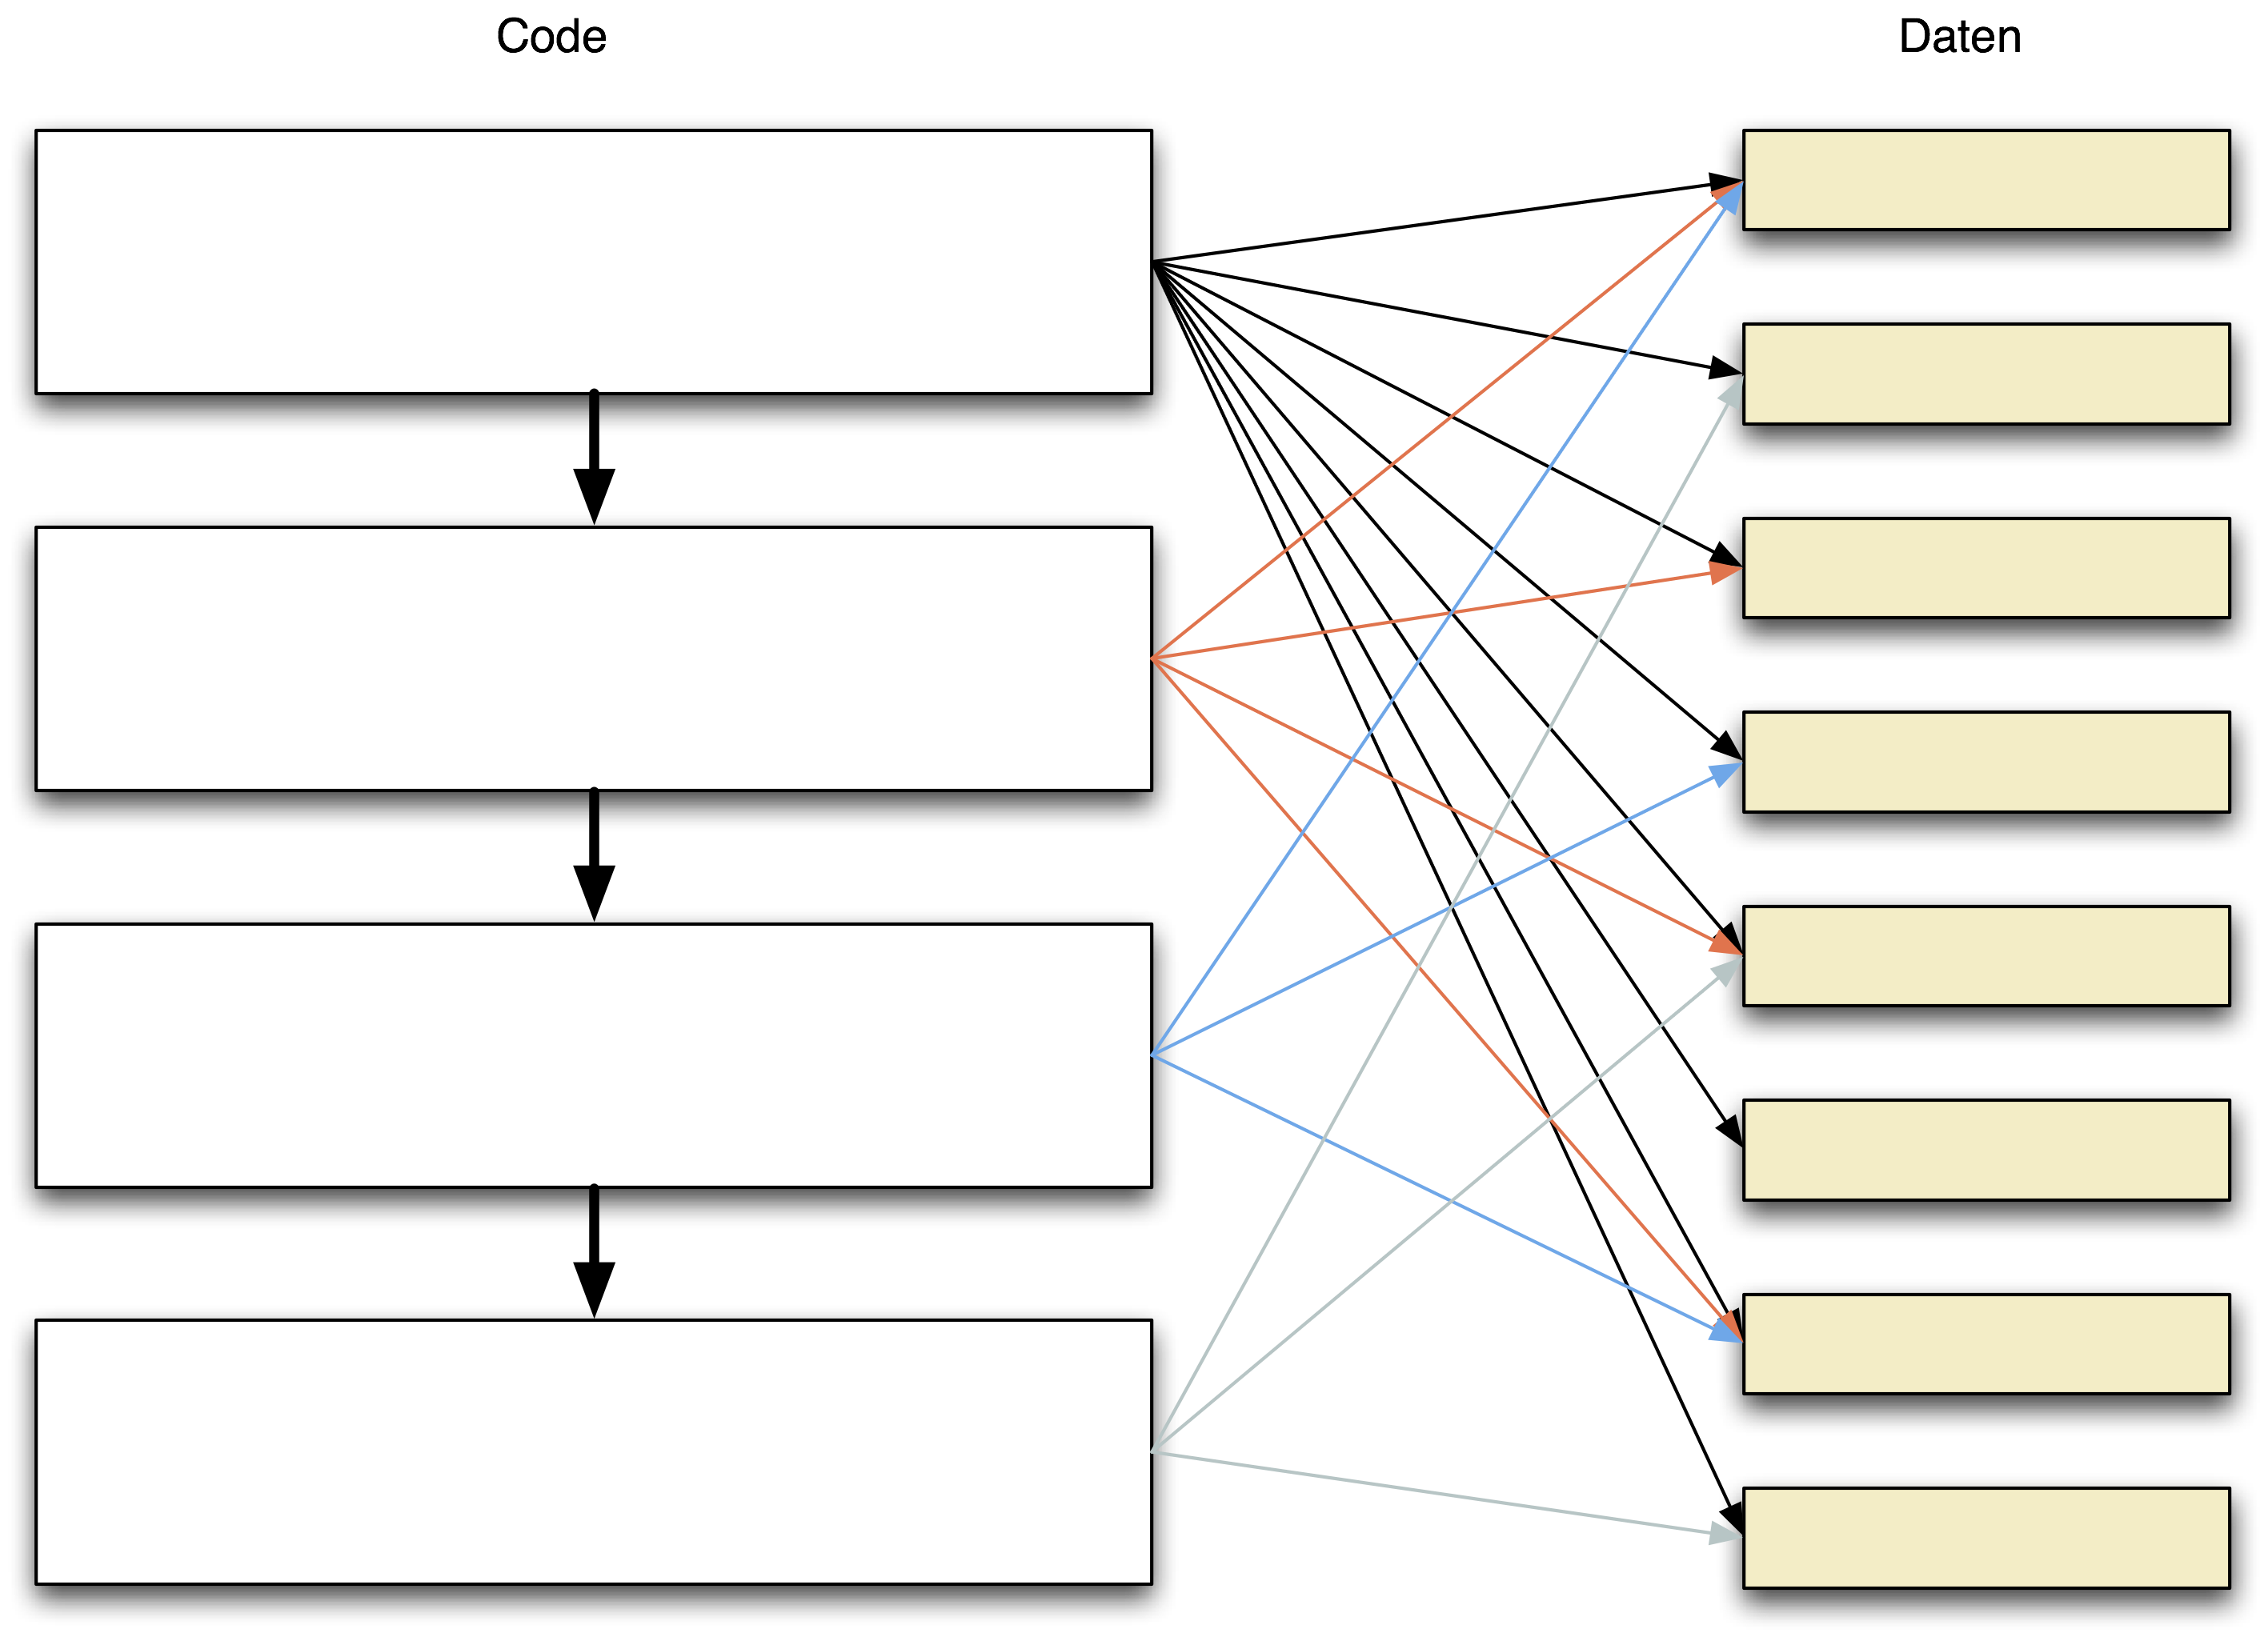
\includegraphics[width=\textwidth]{Codestruktur.png}
\end{minipage}

\end{frame}

%%%%%%%%%%%%%%%%%%%%%%%%%%%%%%%%%%%%%%%%%%%%%%%%%%
\begin{frame}[fragile]{Goal}

\begin{minipage}{.45\paperwidth}
\begin{itemize}
\item Structure:
\begin{itemize}
\item Code reflects the business logic
\end{itemize}
\end{itemize}

\begin{itemize}
\item View \textbf{from the outside}, driven by the expected results:
\begin{itemize}
\item Which values do I need?
\item How is each value calculated?
\item Which categories of results exist? Similarities, differences?
\end{itemize}
\end{itemize}
\end{minipage} \hfill
\begin{minipage}{.45\paperwidth}
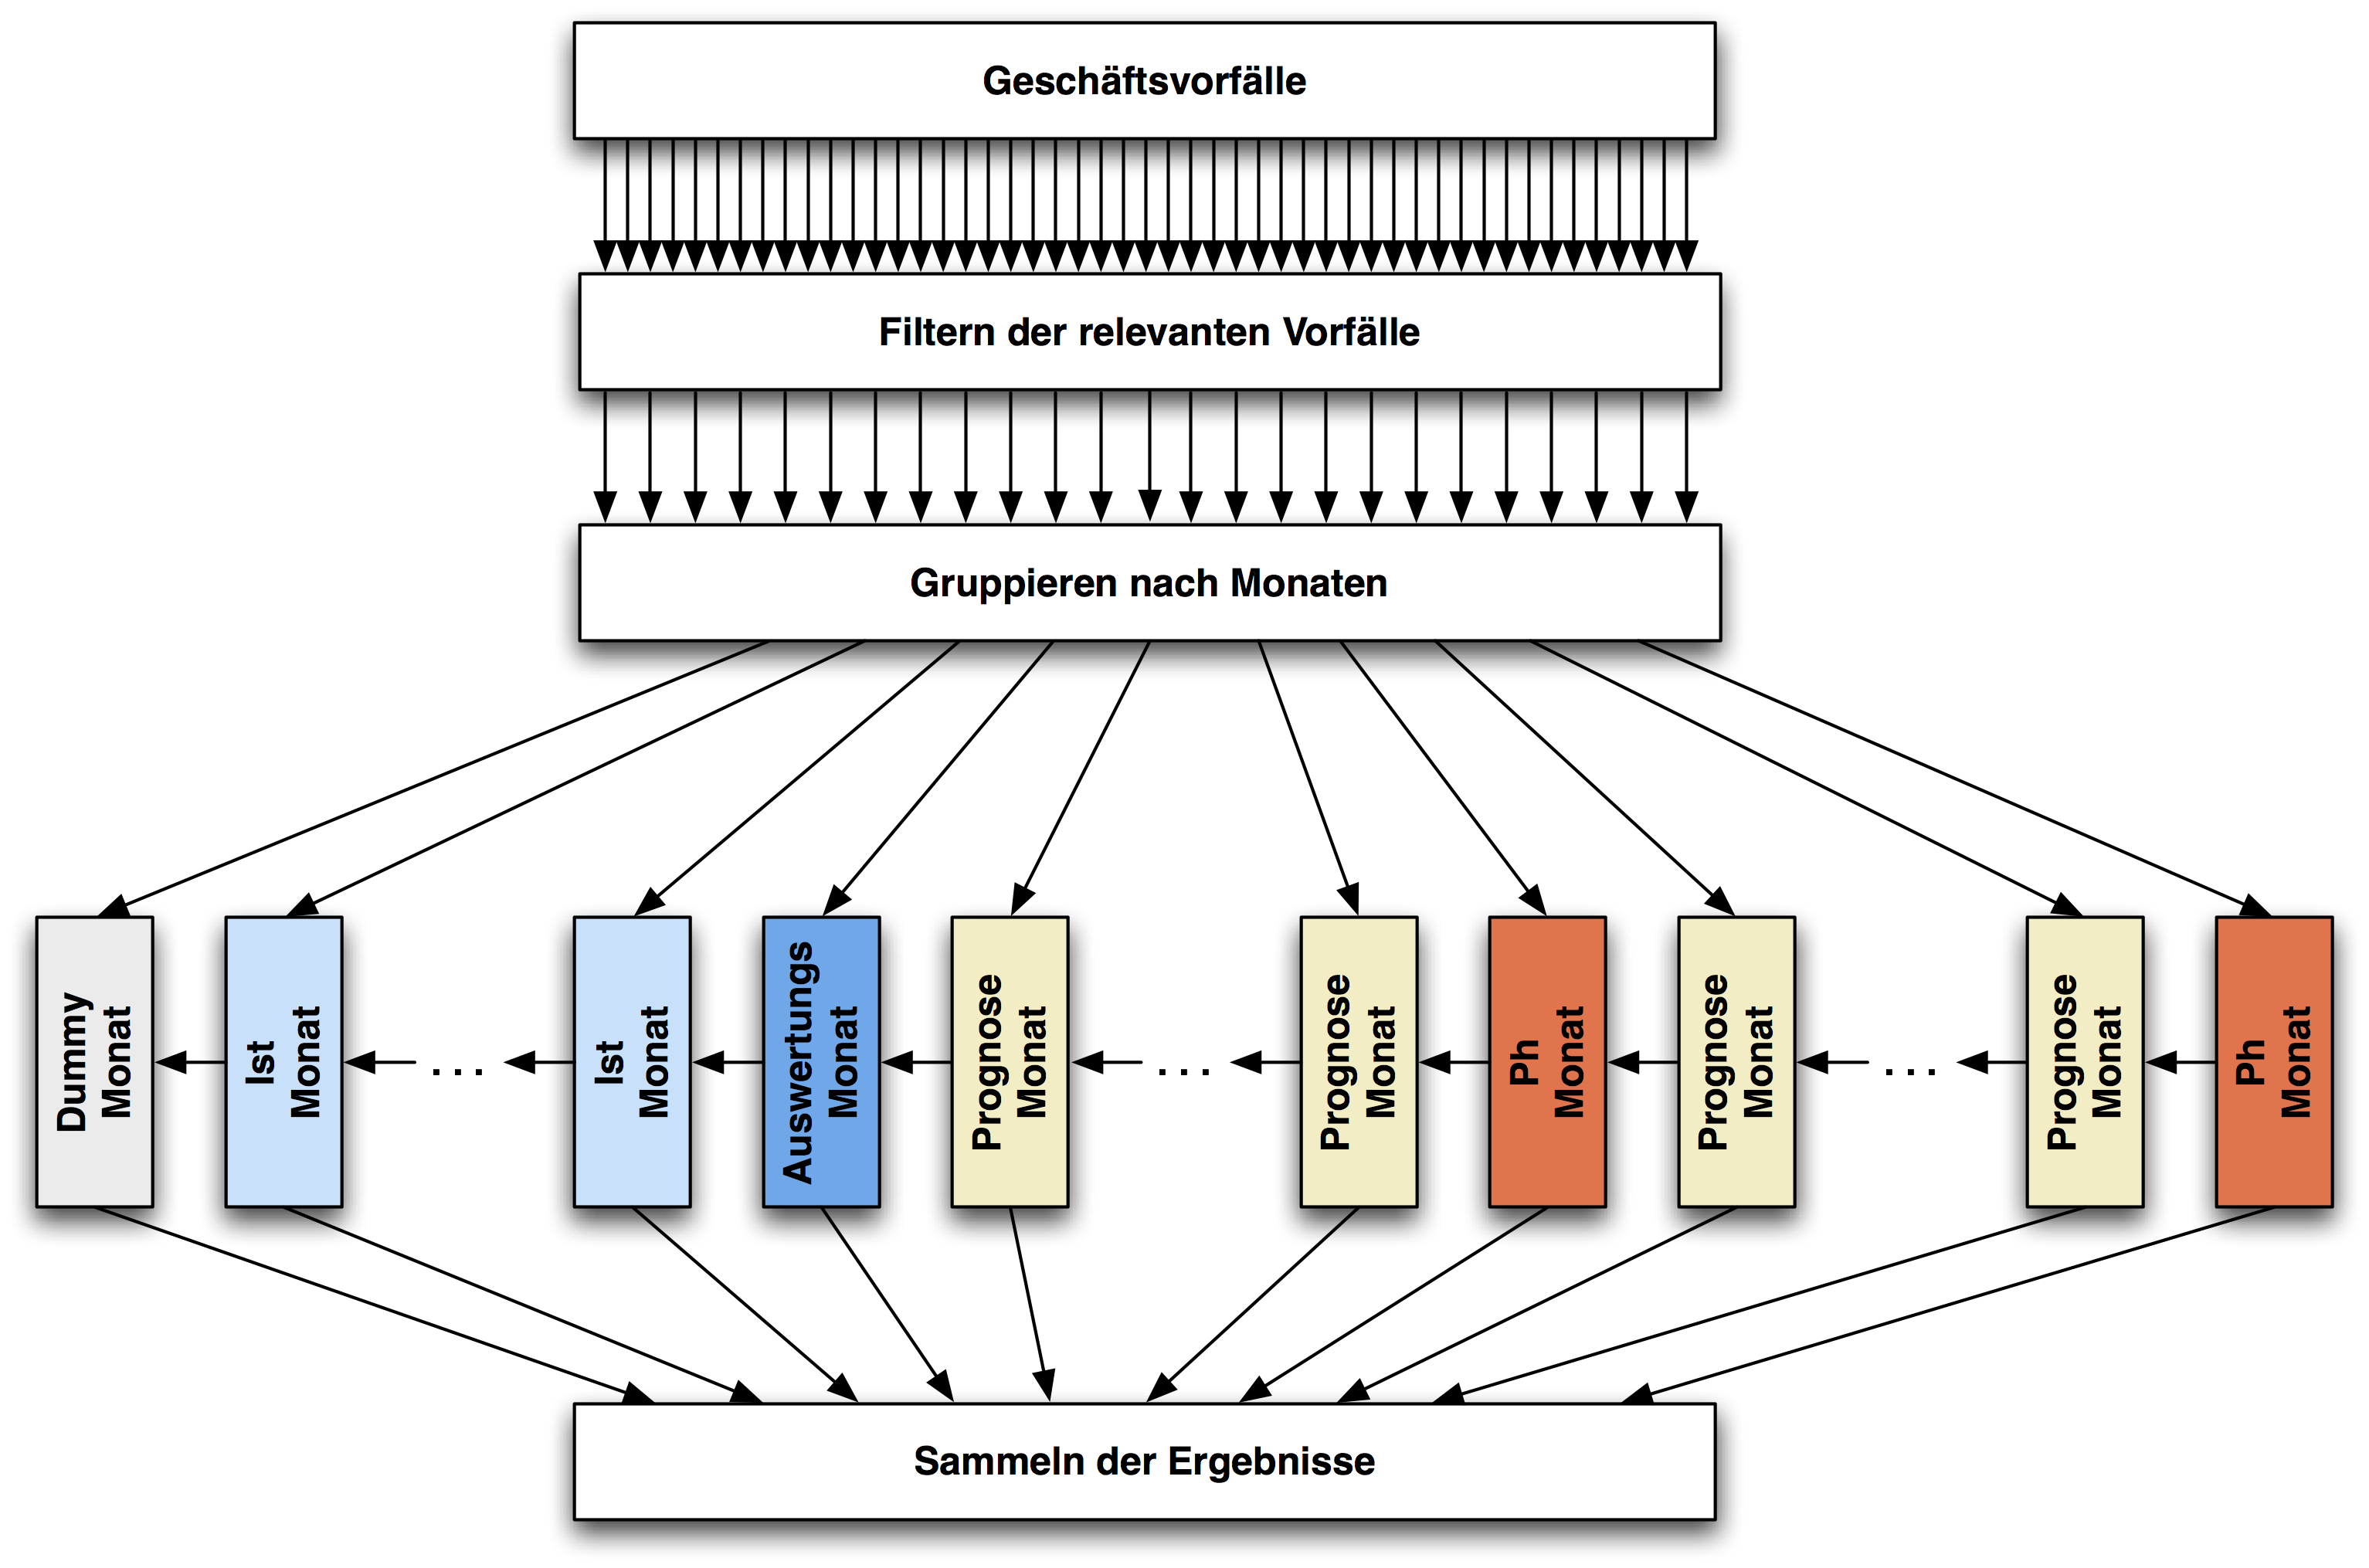
\includegraphics[width=\textwidth]{DynamischFein.jpg}
\end{minipage}

\end{frame}

%%%%%%%%%%%%%%%%%%%%%%%%%%%%%%%%%%%%%%%%%%%%%%%%%%
\begin{frame}[fragile]{Good Approach}
\begin{itemize}
\item Feature-toggle to compare the old and the new version
\begin{itemize}
\item Identification or creation of a minimal entry point to the restructured area
\item The API of this entry point must remain unchanged
\end{itemize}
\end{itemize}

\begin{itemize}
\item Important aspects of the restructuring:
\begin{itemize}
\item Driven by business logic
\item Purely structural (NO changes in behaviour)
\end{itemize}
\end{itemize}

\begin{itemize}
\item Technical goal:
\begin{itemize}
\item Separation of Concerns
\item On-demand-calculation of all values (\glqq Pull\grqq{})
\item Bonus: Value caching via lazy initialization
\end{itemize}

\end{itemize}
\end{frame}

%%%%%%%%%%%%%%%%%%%%%%%%%%%%%%%%%%%%%%%%%%%%%%%%%%
\begin{frame}[fragile]{Important!}
\begin{itemize}
\item If in doubt, the existing code shows the correct behaviour!

\item Do not change the logic while restructuring!

\item Explicit approval of the restructuring
\begin{itemize}
\item It must show identical behaviour (tests, bugs, features)
\end{itemize}

\end{itemize}
\end{frame}

%%%%%%%%%%%%%%%%%%%%%%%%%%%%%%%%%%%%%%%%%%%%%%%%%%
\begin{frame}[fragile]{First Glimpse at the Code}

\begin{center}
{\large \url{00Push/src/push/PushingBalancesCalculator.java}}
\end{center}
\end{frame}

%%%%%%%%%%%%%%%%%%%%%%%%%%%%%%%%%%%%%%%%%%%%%%%%%%
\begin{frame}[fragile]{Quick Poll}

\begin{itemize}
\onslide+<1>
\item Can we improve the code?
\onslide+<2>
\item Is the code readable and understandable?
\onslide+<3>
\item Can you explain how it works?
\end{itemize}

\end{frame}

%%%%%%%%%%%%%%%%%%%%%%%%%%%%%%%%%%%%%%%%%%%%%%%%%%
\begin{frame}[fragile]{Local Optimum}

{
\begin{center}
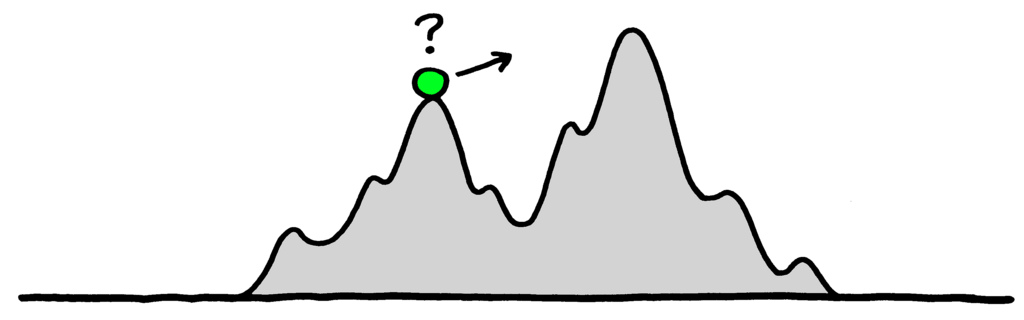
\includegraphics[width=\textwidth]{LocalOptimum.jpg}
\end{center}
\vspace{-1.7em}
\hfill \tiny{\url{https://www.flickr.com/photos/jurgenappelo/5201851938}}
}

\onslide+<2->
\vspace{2em}
Make it worse to be able to improve!

\end{frame}

%%%%%%%%%%%%%%%%%%%%%%%%%%%%%%%%%%%%%%%%%%%%%%%%%%
\begin{frame}[fragile]{Pattern Application - Code Structure}

\begin{itemize}
\item a sequence of input data elements
\item very few classes with logic
\item a sequence of output data elements 
\item output sequence is constructed early in the program run
\item output sequence is filled during program run
\end{itemize}

\end{frame}

%%%%%%%%%%%%%%%%%%%%%%%%%%%%%%%%%%%%%%%%%%%%%%%%%%
\begin{frame}[fragile]{Pattern Application - Code Workflow}

The basic mechanics of the logic class(es) is as follows:

\begin{itemize}
\item initially, the sequence of output data is not filled
\item the main logic part consists of two interlaced loops: 
\begin{itemize}
\item the outer loop iterates over the sequence of output data objects
\item the inner loop iterates over the sequence of input data objects and calculates the data for one output data object
\item at the end of the inner loop, the calculated data is written to that output data object (``push'')
\end{itemize}
\item finally, the sequence of output data is filled
\item the logic class(es) may contain multiple of these interlaced loops in sequence, where a subsequent loop may access and modify the output data that a previous loop has calculated and pushed to the sequence of output data
\end{itemize}

\end{frame}


%%%%%%%%%%%%%%%%%%%%%%%%%%%%%%%%%%%%%%%%%%%%%%%%%%
\begin{frame}[fragile]{Workshop Restrictions \& Rules}

\begin{itemize}
\item Change one thing at a time.
\item Do not change the outside world (i.e.~\texttt{...\_API} classes), only the internals of our calculator class.
\item The code has tests. Run them frequently!
\end{itemize}

\end{frame}




%%%%%%%%%%%%%%%%%%%%%%%%%%%%%%%%%%%%%%%%%%%%%%%%%%
\begin{frame}[fragile]{Workshop Structure}


\begin{enumerate}
\item Disentangle the for loops, isolate the loop body and extract it
\item Build one data object for each loop iteration (instead of reusing the same object over and over again)
\item Isolate the calculations of the distinct values into separate methods and calculate them on demand
\end{enumerate}

\end{frame}



%%%%%%%%%%%%%%%%%%%%%%%%%%%%%%%%%%%%%%%%%%%%%%%%%%
\begin{frame}[fragile]{Workshop}

\begin{center}
{\huge Workshop}
\end{center}
\end{frame}

%%%%%%%%%%%%%%%%%%%%%%%%%%%%%%%%%%%%%%%%%%%%%%%%%%
\begin{frame}[fragile]{Balance}
\begin{center}
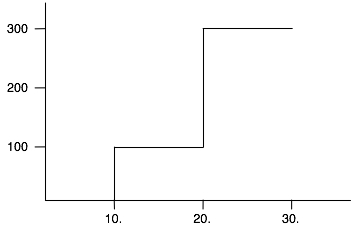
\includegraphics[width=.85 \paperwidth]{../workshopMaterial/balance.jpg}
\end{center}
\end{frame}

%%%%%%%%%%%%%%%%%%%%%%%%%%%%%%%%%%%%%%%%%%%%%%%%%%
\begin{frame}[fragile]{Initial Average}
\begin{center}
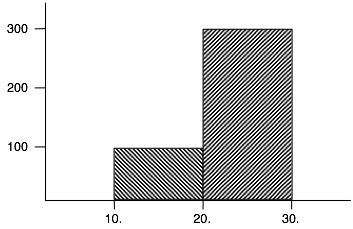
\includegraphics[width=.85 \paperwidth]{../workshopMaterial/initialAverage.jpg}
\end{center}
\end{frame}

%%%%%%%%%%%%%%%%%%%%%%%%%%%%%%%%%%%%%%%%%%%%%%%%%%
\begin{frame}[fragile]{Final Average}
\begin{center}
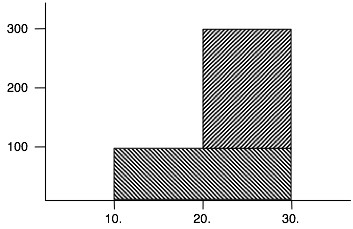
\includegraphics[width=.85 \paperwidth]{../workshopMaterial/finalAverage.jpg}
\end{center}
\end{frame}

%%%%%%%%%%%%%%%%%%%%%%%%%%%%%%%%%%%%%%%%%%%%%%%%%%

%%%%%%%%%%%%%%%%%%%%%%%%%%%%%%%%%%%%%%%%%%%%%%%%%%
{
\begin{frame}{Thank you!}

        Code \& slides at GitHub:
        \begin{center}
                \url{https://github.com/NicoleRauch/RefactoringLegacyCode}
        \end{center}

        \begin{block}{Nicole Rauch}
        \begin{description}[Twitterxx]
                \item[E-Mail]  \href{mailto:info@nicole-rauch.de}{\texttt{info@nicole-rauch.de}}
                \item[Twitter] \href{http://twitter.com/NicoleRauch}{\texttt{@NicoleRauch}}
        \end{description}
        \end{block}
\end{frame}
}
